\documentclass[12pt, UTF8]{article}
\usepackage[a4paper, scale = 0.8]{geometry}
\usepackage{ctex}

\usepackage{enumitem}
\usepackage{listings}
\usepackage{xcolor}
\usepackage{color}
\definecolor{GrayCodeBlock}{RGB}{241, 241, 241}
\definecolor{BlackText}{RGB}{0, 0, 0}
\definecolor{RedTypename}{RGB}{182, 86, 17}
\definecolor{GreenString}{RGB}{96, 172, 57}
\definecolor{PurpleKeyword}{RGB}{184, 84, 212}
\definecolor{GrayComment}{RGB}{170, 170, 170}
\definecolor{GoldDocumentation}{RGB}{180, 165, 45}
\lstset {
  columns = fullflexible, keepspaces = true, showstringspaces=false, breaklines = true, frame = single, framesep = 0pt, framerule = 0pt, framexleftmargin = 4pt, framexrightmargin = 4pt, framextopmargin = 5pt, framexbottommargin = 3pt, xleftmargin = 4pt, xrightmargin = 4pt,
  backgroundcolor = \color{GrayCodeBlock},
  basicstyle = \ttfamily\color{BlackText},
  keywordstyle = \color{PurpleKeyword},
  ndkeywordstyle = \color{RedTypename},
  stringstyle = \color{GreenString},
  commentstyle = \color{GrayComment}
}

\usepackage{graphicx}
\usepackage{amsmath}

\usepackage[colorlinks, linkcolor = red, anchorcolor = blue, citecolor = green]{hyperref}

\renewcommand\thesection{\arabic{section}}

\title{数据挖掘第四次作业}
\author{李晨昊 2017011466}
\begin{document}
\maketitle

\section{数据立方体练习}

假定某一数据仓库包含4个维:date(日期),spectator(观众),location(地点)和game(节目);2个度量count和charge,count是观众的人数,charge是观众在某日期某地点观看某节目的费用。观众分三类:学生、成年人和老人,每类观众有不同的收费标准。
\begin{enumerate}
  \item 画出该数据仓库的星型模式图StarSchema(自己定义维表属性)(2分)。

  \begin{center}
    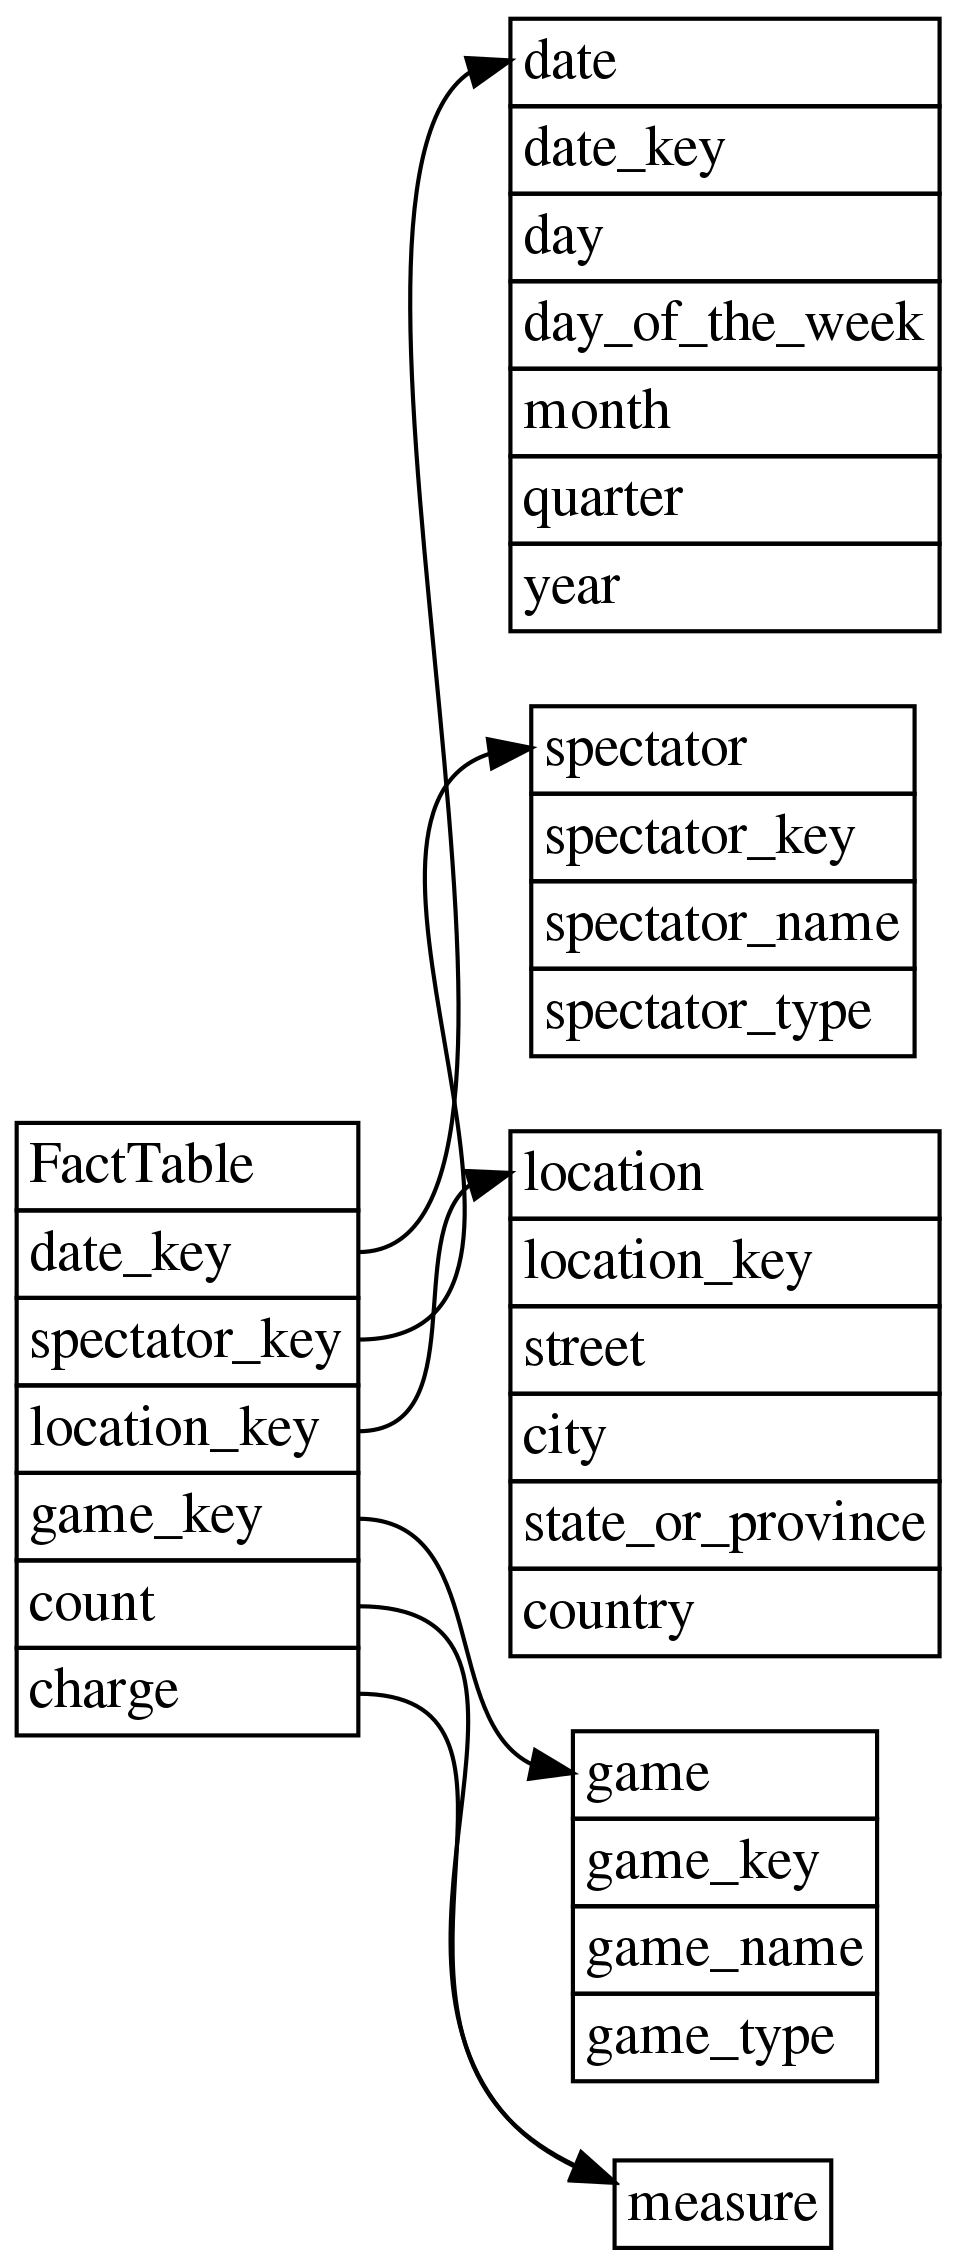
\includegraphics[width=0.22\textwidth]{t1.png}
  \end{center}
  
  \item 从基本方体[date, spectator, location, game]开始,为列出2018年学生观众在清华大学大礼堂的总付费,应当执行哪些OLAP操作,并说明原因(2分)。
  
  \begin{enumerate}
    \item drill-down on spectator to spectator\_type
    \item drill-down on date to year
    \item drill-down on location to street
    \item dice for spectator\_type=学生 and date=2018 and location=清华大学大礼堂
  \end{enumerate}

  原因:需要先执行drill-down讲需要检测的维度暴露出来,然后用dice讲需要的数据方块选择出来。
\end{enumerate}

\section{频繁项集挖掘}

\begin{table}[htbp]
\begin{center}
  \begin{tabular}{|c|c|}
    \hline
    TID & Items \\ \hline
    1   & ABC   \\ \hline
    2   & ABCD  \\ \hline
    3   & BCE   \\ \hline
    4   & ACDE  \\ \hline
    5   & DE    \\ \hline
  \end{tabular}
\end{center}
\end{table}

\begin{enumerate}
  \item 写出表1中事务数据集的极大频繁项集(最小支持度为2)(2分)。
  
  $\{CE, DE, ABC, ACD\}$
  \item 写出表1中事务数据集的闭频繁项集(最小支持度为2)(2分)。
  
  $\{C, D, E, AC, BC, CE, DE, ABC, ACD\}$
  \item 简述频繁项集、极大频繁项集和闭频繁项集之间的关系(2分)。
  
  极大频繁项集是闭频繁项集的子集,闭频繁项集是频繁项集的子集。
\end{enumerate}

\end{document}
